\documentclass[12pt, twoside]{article}
\usepackage[letterpaper, margin=1in, headsep=0.5in]{geometry}
\usepackage[english]{babel}
\usepackage[utf8]{inputenc}
\usepackage{amsmath}
\usepackage{amsfonts}
\usepackage{amssymb}
\usepackage{tikz}
\usepackage{yhmath}
\usetikzlibrary{quotes, angles}
\usepackage{graphicx}
\usepackage{enumitem}
\usepackage{multicol}

\newif\ifmeta
\metatrue %print standards and topics tags

\title{Regents Geometry}
\author{Chris Huson}
\date{March 2022}

\usepackage{fancyhdr}
\pagestyle{fancy}
\fancyhf{}
\renewcommand{\headrulewidth}{0pt} % disable the underline of the header
\raggedbottom

\fancyhead[LE]{\thepage}
\fancyhead[RO]{\thepage \\ Name: \hspace{4cm} \,\\}
\fancyhead[LO]{BECA / Dr. Huson / Geometry\\* Unit 8: Circles\\* 9 March 2022}

\begin{document}
\subsubsection*{8.5 Pre-Exam: Area, volume, solids, circles review}
\emph{Unless otherwise instructed, find an exact answer, in terms of $\pi$ or using radicals if necessary.}
 \begin{enumerate}

  \item Use the formulas for the area and circumference of circles:
  \[A=\pi r^2\]
  \[C=\pi D = 2\pi r\]
  
  \item Given the circle centered at $O$ with radius $r=3$. Leave an exact answer, in terms of $\pi$ if necessary.
  \begin{multicols}{2}
    \begin{enumerate}
      \item Find the circumference of circle $O$. %\vspace{1cm}
      \item Find the area of the circle.\vspace{2cm}
    \end{enumerate}
    %\columnbreak
    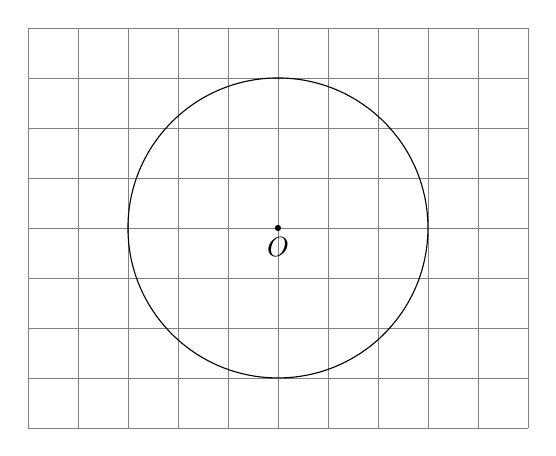
\begin{tikzpicture}[scale=.635]
      \draw [help lines] (-5,-4) grid (5,4);
      %\draw [thick, ->] (-2.2,0) -- (10.4,0) node [below right] {$x$};
      %\draw [thick, ->] (0,-2.2)--(0,10.4) node [left] {$y$};
      \draw (0,0) circle [radius=3] node[below]{$O$};
      \draw [fill] (0,0) circle [radius=0.05];
    \end{tikzpicture}
  \end{multicols}

  \item Find the radius of a circle having an area of $25 \pi$. \vspace{2cm}
  
  \item Find the area of the shape shown below composed of a rectangle and circular cap. Leave your answer as an exact value in terms of $\pi$.
    \begin{flushright}
    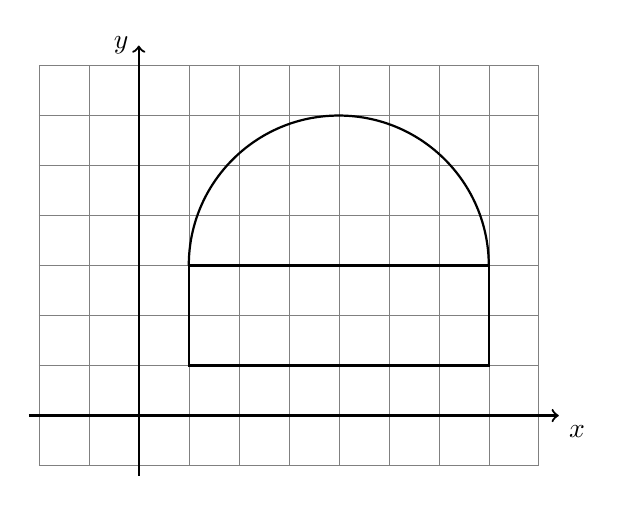
\begin{tikzpicture}[scale=.635]
      \draw [help lines] (-2,-1) grid (8,7);
      \draw [thick, ->] (-2.2,0) -- (8.4,0) node [below right] {$x$};
      \draw [thick, ->] (0,-1.2)--(0,7.4) node [left] {$y$};
      \draw [thick] (1,1)--(7,1)--(7,3)--(1,3)--cycle;
      %\draw [thick] (3,4) arc (90:270:1);
      \draw [thick] (7,3) arc (0:180:3);
    \end{tikzpicture}
  \end{flushright}\vspace{1cm}

\newpage
\item A regular heptagon (7 sides) is inscribed in circle $O$, having a radius $r=3$.
    \begin{multicols}{2}
    \raggedcolumns
    \begin{enumerate}[itemsep=1.5cm]
      \item Find the area of the sector $AOB$.
      \item Find the perimeter of sector $AOB$. %\vspace{1.5cm}
      \item Find the measure of central angle $\angle AOB$
    \end{enumerate}
    \begin{flushright}
      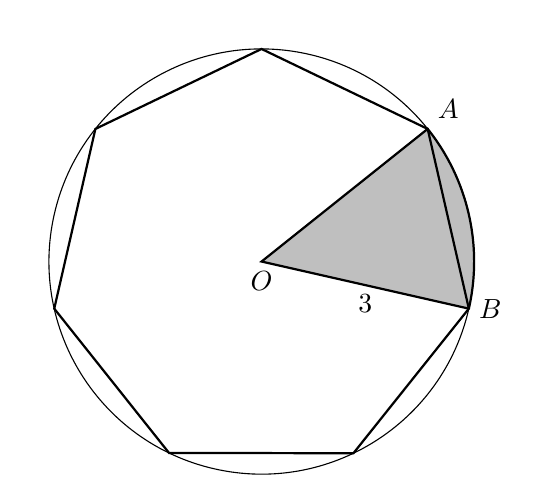
\begin{tikzpicture}[scale=0.9, rotate=-12.8]
        \draw (0,0) circle[radius=3];
        \fill [lightgray]
        (0,0)--(0:3) arc (0:51.4:3)--(0,0);
        \draw [thick]
        (0:3) node[right] {$B$}--
        (0,0) node[below] {$O$}--
        (51.4:3) node[above right] {$A$} arc (51.4:0:3);
        \draw (1.5,0) node[below] {$3$};
        %\draw [thick] (0:3)--(72:3)--(2*72:3)--(3*72:3)--
        %(4*72:3)--cycle;
        \draw [thick] (0:3)--(51.4:3)--(2*51.4:3)--(3*51.4:3)--
        (4*51.4:3)--(5*51.4:3)--(6*51.4:3)--cycle;
      \end{tikzpicture}
    \end{flushright}
    \end{multicols}

    \vspace{1cm}

    \item Given the circle with center $P$ with central angle $\angle APB$ and inscribed angle $\angle AQB$. The intercepted arc has a measure $m \wideparen{AB}=82^\circ$.
  \begin{multicols}{2}
    \raggedcolumns
    \begin{enumerate}
      \item Find $m\angle APB=$ \vspace{0.7cm}
      \item Find $m\angle AQB=$ \vspace{0.7cm}\\
      Circle True or False:
      \begin{enumerate}[itemsep=0.3cm]
        \item T \, F \, $\overline{AP}$ is a radius
        \item T \, F \, $\overline{AQ}$ is a diameter
        \item T \, F \, $\angle AQB$ is an inscribed angle
      \end{enumerate}
    \end{enumerate}
      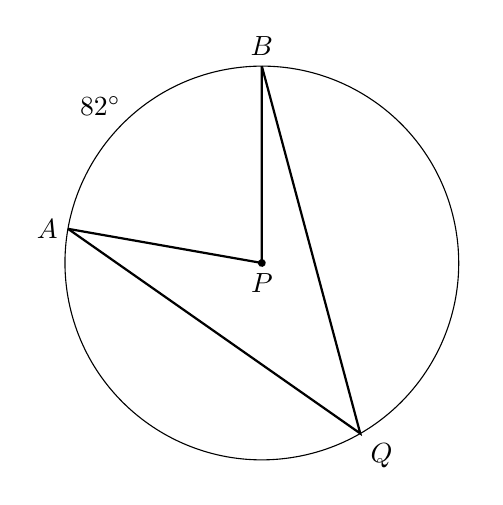
\begin{tikzpicture}[rotate=100, scale=.5]
        \draw (0,0) circle[radius=5];
        \fill (0,0) circle[radius=0.1];
        \draw [thick]
        (-10:5) node[above] {$B$}--
        (0,0) node[below] {$P$}--
        (70:5) node[left] {$A$};
        \draw [thick] (-10:5)--(200:5) node[below right] {$Q$}--(70:5);
        \draw (30:5.2) node[left]{$82^\circ$};
      \end{tikzpicture}
  \end{multicols} \vspace{0.5cm}

  \item Given $R(-3,1)$ and $S(5,7)$, find the length of $\overline{RS}$. Note: $l=\sqrt{(x_2-x_1)^2+(y_2-y_1)^2}$. %\vspace{4cm}
  
\newpage
  \item Perform each calculation, writing down the full calculator display and then rounding to the \emph{nearest hundredth}.
  \begin{multicols}{2}
  \begin{enumerate}
    \item $V=\frac{1}{3} \pi (2.4)^2(5.1)$
    \item $P=3.6 + \frac{1}{2} \pi (3.6)$  
  \end{enumerate}
  \end{multicols}\vspace{2cm}

  \item Solve each equation for the appropriate variable. Do not round. Simplify radicals.
  \begin{multicols}{2}
  \begin{enumerate}[itemsep=2cm]
    \item $A=\pi r^2=27\pi$
    \item $V=\frac{1}{3}(6.0)^2h=153$  
  \end{enumerate}
  \end{multicols}\vspace{5cm}

  \subsubsection*{Model the situation with an equation. Use the formula sheet. You must start with a labeling variable. \hfill Do NOT solve!}

  \item A large concrete post in the shape of a cylinder has a volume of 250 cubic feet. Its height is 12 feet. Find the radius of the base of the post. \vspace{2cm}

  \item A spherical cork fishing net float has a volume of 4000 cubic centimeters. Find its radius. \vspace{2cm}

  \item The volume of a cone having a \textbf{diameter} of 10 inches is 200 cubic inches. Find the cone's height. \vspace{2cm}

  \newpage
  \subsubsection*{Applying density ratios}
  \item A tank of gasoline holds 15 gallons. Find the cost to completely fill the tank if gasoline costs \$3.15 per gallon. \vspace{3cm}
  \item A stick of butter has a volume of 90 cubic centimeters. If the density of butter is 0.9 grams per cubic centimeter, find the weight of a stick of butter. \vspace{3cm}
  \item A large glass marble has a diameter of 3 cm. The density of glass is 2.70 $\mathrm{g/cm}^3$. Find the weight of the marble. \vspace{3cm}

  \item A bar of solid gold is in the shape of a rectangular prism having a length of 12 cm, width of 2 cm, and thickness of 2 cm. The density of gold is 19.3 grams per cubic cm, and its approximate market value is \$50 per gram.
  \begin{enumerate}
    \item Find the weight of the bar of gold.  \vspace{3cm}
    \item Find its value in dollars.
  \end{enumerate}

\newpage
  \item Perform each calculation, writing down the full calculator display and then rounding to the \emph{nearest hundredth}.
    \begin{multicols}{2}
    \begin{enumerate}[itemsep=4cm]
      \item $A=15.944732$
      \item $W=3.4 \times 9.8 \times 4.3 \times 0.15$
            
      \item $V=\frac{1}{3} \pi (3.4)^2(6.1)$
      \item $P=8.6 + \frac{1}{2} \pi (8.6)$  
      \item $V=199.19711$
      \item $W=\frac{1}{3} (13)  3.3^2 \times 1.175$
      \item $V=\frac{1}{3} \pi (12.4)^2(8.1)$
      \item $P=12 + \frac{1}{4} \pi (12)$ 
    \end{enumerate}
    \end{multicols}\vspace{2cm}


\end{enumerate}
\end{document}
